% ---------------------------------------
% section : Event Triggering
% ---------------------------------------
\section{Trigger System}
\label{sec:cmsexperiment:trigger}

% overview
CMS applies a two-tiered trigger system \cite{cms:trigger:Khachatryan:2016bia} to select the events of interest. The \acrfull{l1t}, composed of custom hardware processors, uses information from the calorimeters and muon detectors to reduce the event rate from 40~MHz to 100~kHz, within a latency less than 4~$\mu s$. The second level, known as the \acrfull{hlt}, consists of a farm of processors running a version of the full event reconstruction software optimized for fast processing. The HLT further reduces the event rate from 100 kHz to 1 kHz and output for data storage.



\subsection{Level-1 Trigger}

\begin{figure}[ht]
    \centering
    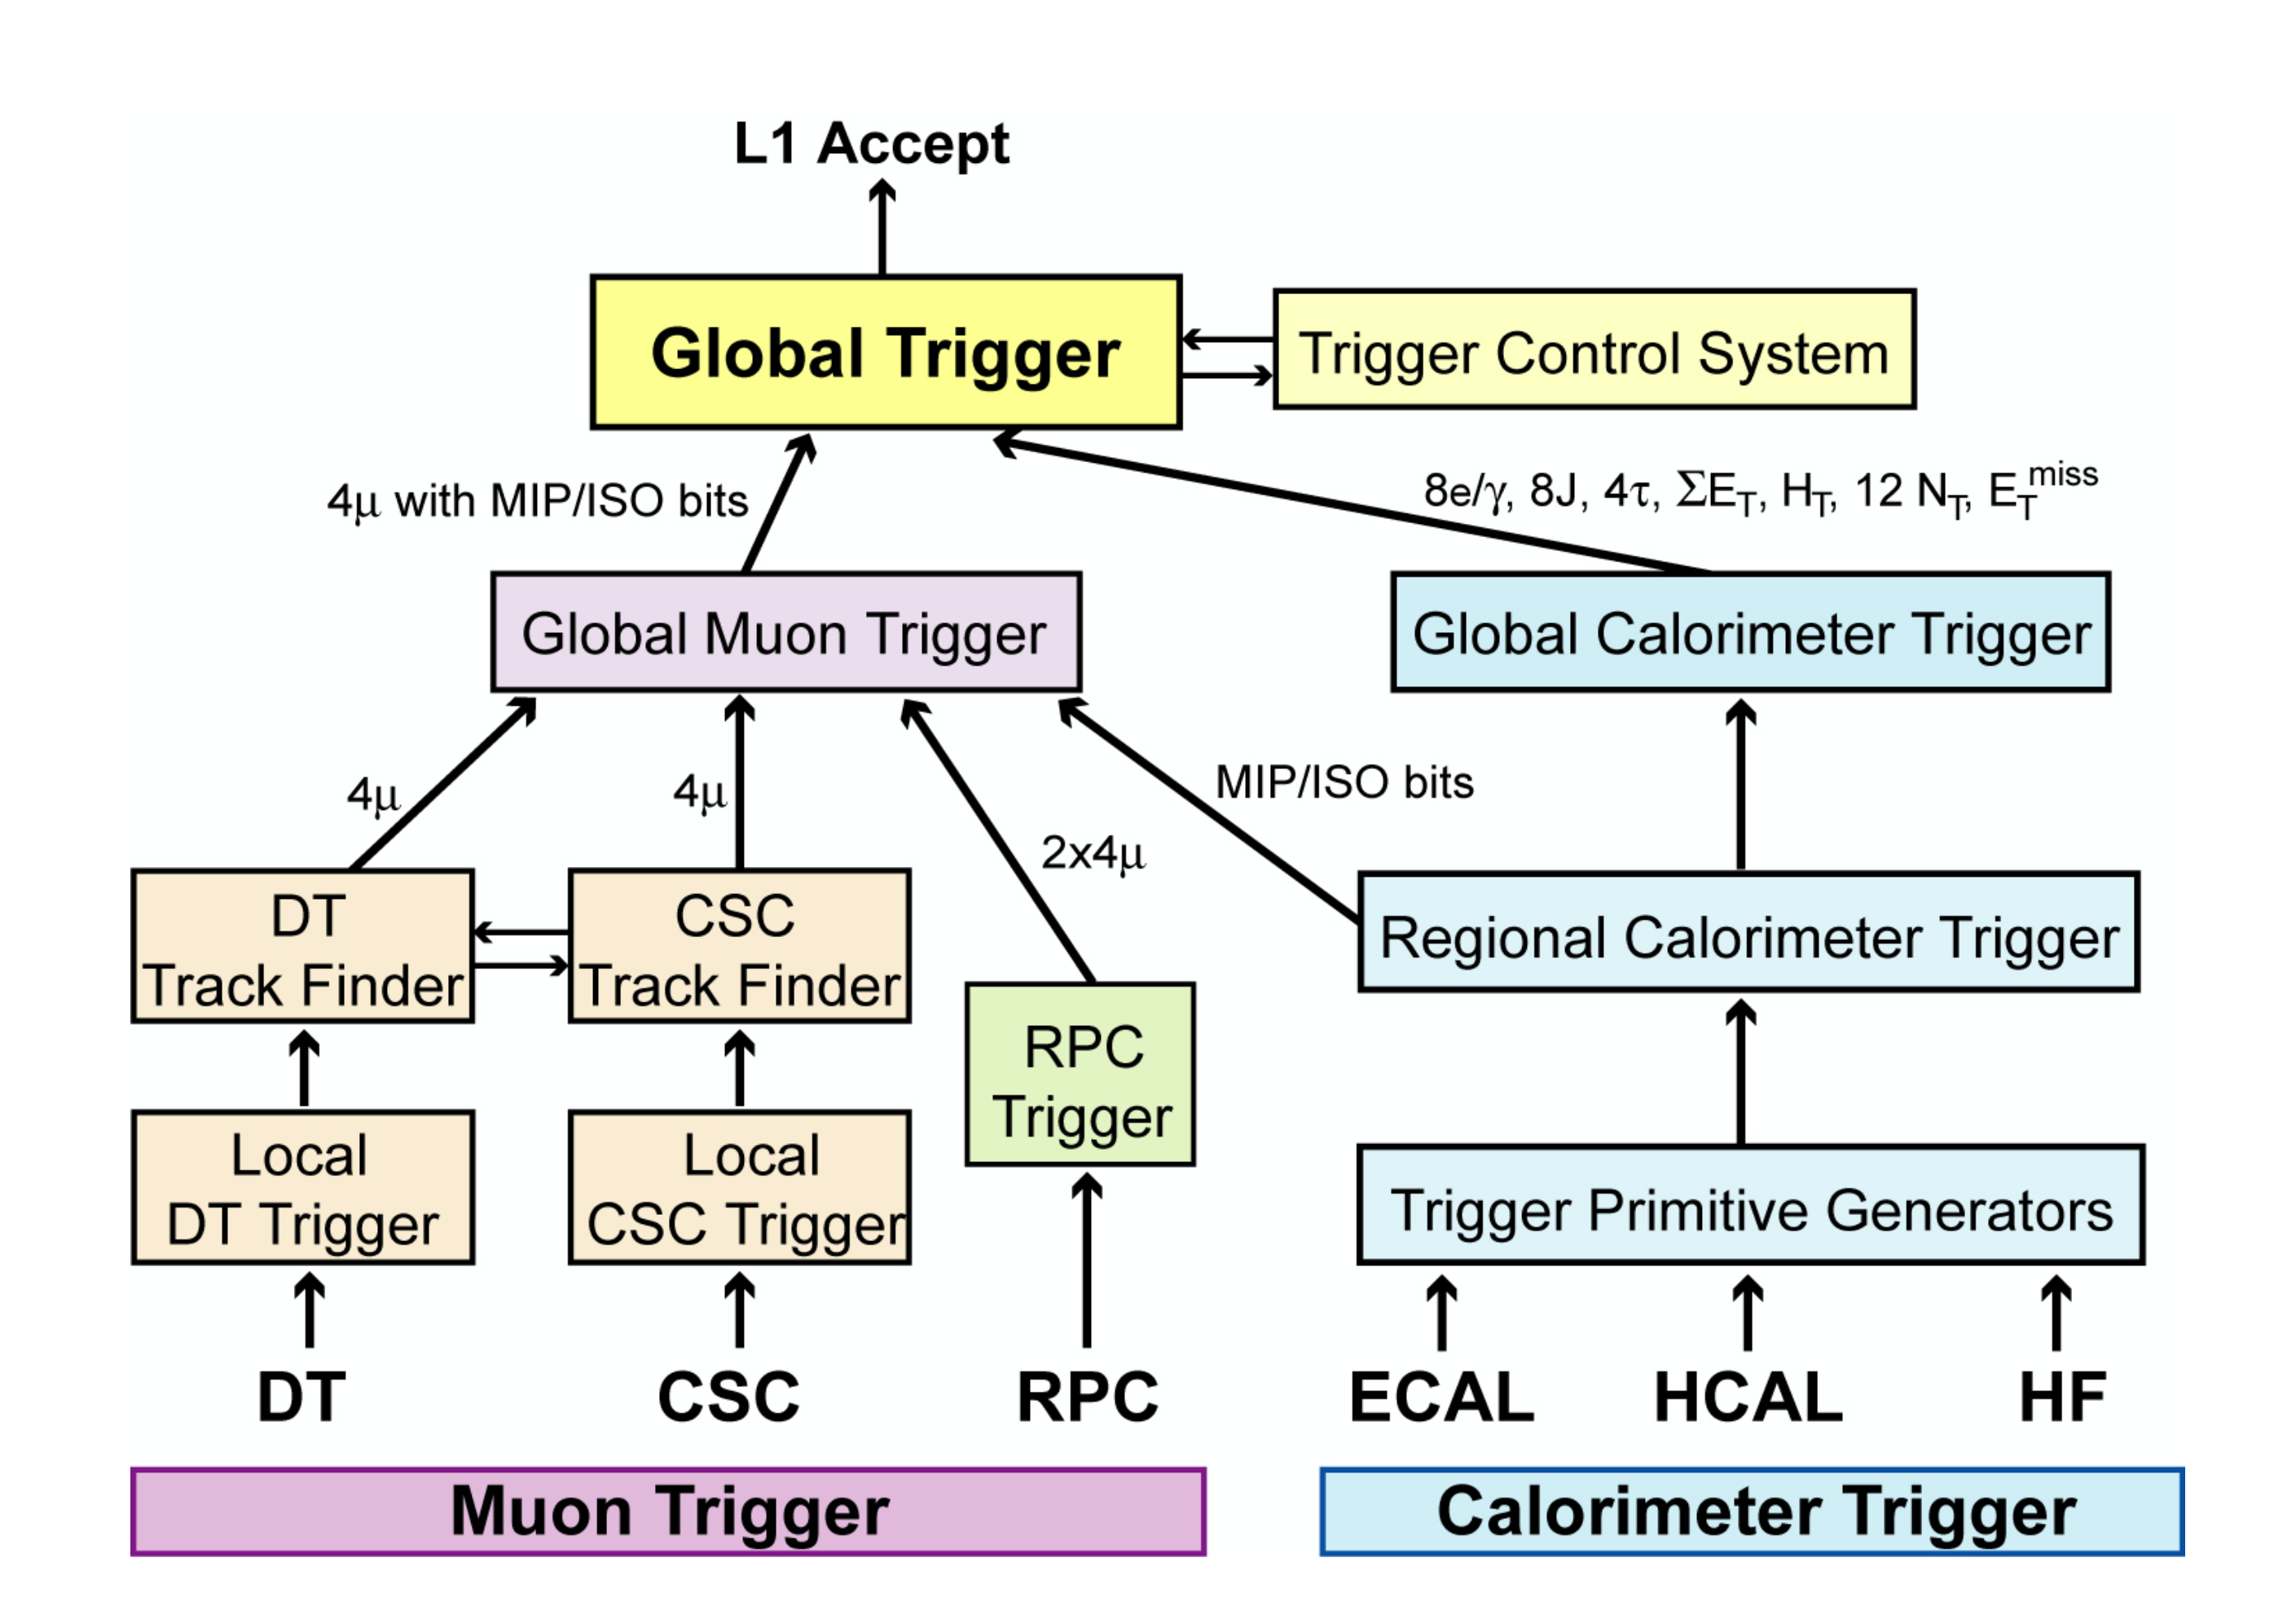
\includegraphics[width=0.8\textwidth]{chapters/CMSExperiment/sectionTrigger/figures/trigger.png}
    \caption{The logic structure of L1T.}
    %  Calorimeters and muon detectors raise local trigger primitives to compute a regional trigger signal. Then \acrfull{gmt} summarizes regional information from DT, SCS and PRC, while \acrfull{gct} concentrates the regional information from ECAL, HCAL and HF. Finally \acrfull{gt} makes the final decision based on the object orientated information from GMT and GCT and transport data in the sub-detectors to the HLT if L1T accept is made. 
    \label{fig:cmsexperiment:trigger:structure}
\end{figure}

% overview
L1 Trigger is designed to cope with the high collision frequency in the LHC, reducing the event rate from 40~MHz to 100~kHz, keeping only potential events of physics interest. To achieve this, the L1 trigger is designed with three components: local, regional, and global trigger. The logic structure is shown in Figure~\ref{fig:cmsexperiment:trigger:structure}. The local triggers, also called \acrfull{tpg}, are based on energy deposits in the calorimeter trigger towers as well as the track segments or hit patterns in muon chambers. Regional triggers combine the information from the local triggers in limited regions. They use pattern logic to determine the sorted trigger objects, such as electron or muon candidates. The \acrfull{gct} and \acrfull{gmt} determine the highest-rank calorimeter and muon objects across the entire experiment and transfer them to the \acrfull{gt}, the top entity of the Level-1 hierarchy. GT decides to reject an event or to accept it for further evaluation by the HLT. The Level-1 Accept decision is communicated to the sub-detectors through the \acrfull{ttc} system. Before decisions reach the front-end, the raw data are stored in FIFO pipelined memories in the front end electronics. Limited by the memory size, only a latency of \SI{3.2}{\us} is allowed between a given bunch crossing and the distribution of the L1T decision to the detector front-end electronics. The L1T electronics are housed partly on the detectors, partly in the underground control room located at approximately 90~m from the experimental cavern.


% \begin{itemize}
%     \item Calorimeter part. The \acrfull{tpg} make up the local step of the Calorimeter Trigger pipeline. For triggering purposes, the calorimeters are subdivided into trigger towers. Each TPG sums up the transverse energies measured in ECAL crystal tower or HCAL read-out tower to obtain the trigger tower's $E_T$, and then it attaches the correct bunch crossing number. The TPG electronics are integrated with the calorimeter read-out. The TPGs are transmitted through high-speed serial links to the regional calorimeter trigger, which determines regional candidate electrons/photons, transverse energy sums, $\tau$-veto bits, and information relevant for muons in the form of \acrfull{mip} and isolation bits. The Global Calorimeter Trigger determines the highest-rank calorimeter trigger objects across the entire calorimeter system, including 8 $e/\gamma$, 8 jets, 4 $\tau$, $\sum E_T$, $H_T$, 12 $n_j$, met.
    

%     \item Muon part. All three muon systems – the DT, the CSC, and the RPC – take part in the L1T. The barrel DT chambers provide local trigger information in the form of track segments in the $\phi$-projection and hit patterns in the $\eta$-projection. The endcap CSCs deliver 3-dimensional track segments. All chamber types also identify the bunch crossing from which an event originated. The regional muon trigger consists of the DT and CSC track finders, which join segments to complete tracks and assign physical parameters. Besides, the RPC trigger chambers, which have excellent timing resolution, deliver their own track candidates based on regional hit patterns. The Global Muon Trigger then combines the information from the three sub-detectors and outputs 4 leading $\mu$ in the full coverage of the muon system, achieving an improved momentum resolution and efficiency comparing with the stand-alone systems.
    
%     \item Global. The GT decides to accept or reject an event at L1 based on trigger objects delivered by the GCT and GMT. The L1T accept decision is communicated to the sub-detectors through the TTC system. Then raw data corresponding to the triggered bunching crossing is read out from all front-end FIFO memories across the whole detector. The raw data, together with the L1T objects from GT, are sent to the HLT.
% \end{itemize}






\subsection{High Level Trigger}

The event selection at the HLT is performed similarly to that used in the offline processing. For each event, objects such as electrons, muons, jets are reconstructed, and a menu of identification criteria is applied to select the events of physics interest.

% builder-filter
The HLT hardware consists of a CPU processor farm composed of commodity computers, the \acrfull{evf}, running Scientific Linux operating system. The event filter farm consists of thousands of builder-filter units. In the builder units, individual event fragments from the detector are assembled to form complete events. Upon request from a filter unit, the builder unit ships an assembled event to the filter unit. The filter unit then unpacks the raw data into detector-specific data structures and performs the event reconstruction and selection. The associated builder unit and filter unit are located in a single multi-core machine and communicate via a shared memory. In total, the EVF was executed on approximately 13,000 CPU cores at the end of 2012. On average, the HLT processing time per event is about 90~ms. EVF with 13,000 CPU cores allows the L1T output rate up to 100~kHz. With a fixed L1T rate, increasing CPU cores allows HLT to have more time budget per event. The output rate of the HLT is about 1 kHz. The output rate is an optimal choice based on the event size, as well as the computing and storage capacity of the offline system.

% filtering and storage
The HLT filtering process uses the full precision of the data from the detector. The selection is based on offline-quality reconstruction algorithms. It works by computing a menu of the HLT paths, in each of which a predefined process of object reconstruction and event selection is executed. If at least one of the HLT paths get past, the event will be accepted and sent to storage and offline processing. Upon the HLT accept decisions are made, the events are sent to the storage manager for archival storage. The event data are stored locally on disk and eventually transferred to the CMS Tier-0 computing center for offline processing and permanent storage. Events are grouped into a set of non-exclusive streams according to the HLT decisions.
